\section{Anexos}

\begin{frame}{Anexos}
	\begin{alertblock}{Anexos}
	\end{alertblock}
\end{frame}


\begin{frame}{Modelos computacionais baseados em distância}
\selectFont
\begin{tcolorbox}[colback=blue!5!white,colframe=blue!75!black,valign=center,title=Regra $\Delta$ de Burrows ]\selectFont
	\begin{equation}
	\begin{aligned}
	\Delta Burrow \left ( A, B \right) = \frac{1}{N}\sum_{i=1}^{N}\left | Zscore(A_i,C_i) - Zscore(B_i,C_i) \right |
	\\
	Zscore(X_i,C_i)= \frac{X_i - \mu (C_i) }{\sigma(C_i)}
	\end{aligned}
	\label{eq:deltaBorrow}
	\end{equation}
	
	Distância de Manhattan dos Z-score das frequências         
\end{tcolorbox}

A e B são vetores de frequências dos documentos. C é o vetor de frequência do córpus.

\end{frame}

\begin{frame}{Modelos de aprendizado de máquina (AM)}

\begin{columns}
	\begin{column}{0.55\textwidth}
		\begin{tcolorbox}[colback=blue!5!white,colframe=blue!75!black,valign=center,title=Regressão logística softmax]\selectFont
			\centering
			\begin{equation} 
			\begin{matrix}
			f_1(X) - \ln Z  & = \ln P(Y=1|X) \\
			\cdots & \cdots \\
			f_c(X) - \ln Z & = \ln P(Y=c|X) \\
			\end{matrix}
			\label{eq:logisticaArray}
			\end{equation}
			
			$\Downarrow$
			
			\begin{equation}
			P(Y=c|X) =softmax(X,c) = \frac{e^{f_c(X)}}{\sum_{k=1}^{K} e^{f_k(X)}}
			\label{eq:softmax}
			\end{equation}
		\end{tcolorbox}
	\end{column}
	\begin{column}{0.45\textwidth}
		\begin{tcolorbox}[colback=blue!5!white,colframe=blue!75!black,valign=center,title=Propriedades]\selectFont
			$\bullet$ Não assume a independência das variáveis.
			
			$\bullet$ Possui saída probabilística.
			
			$\bullet$ As probabilidades reflem o balanceamento das classes.
			
			$\bullet$ Possui saída contínua.
			
			$\bullet$ É um classificador linear.
			
			$\bullet$ É usado em aprendizado profundo.
		\end{tcolorbox}
	\end{column}
\end{columns}
\end{frame}

\begin{frame}{Modelos de aprendizado de máquina (AM)}
\selectFont
	\begin{figure}[H]\centering
		\caption{Arquitetura de convolução para sentenças e documentos}\selectFont
		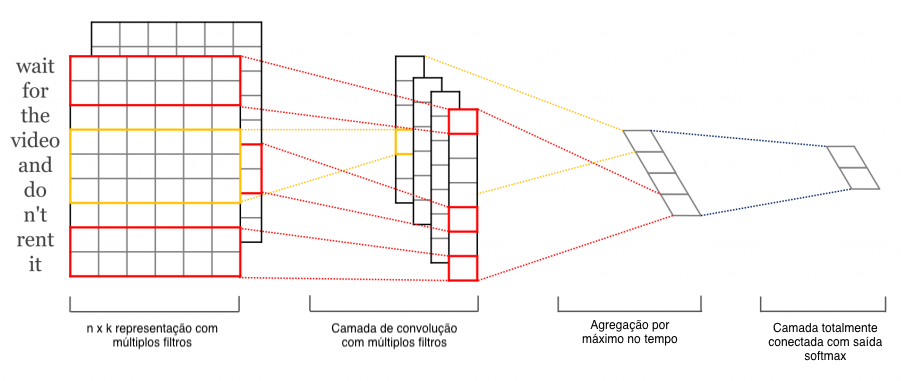
\includegraphics[scale=0.27,origin=c,]{images/CNNKIN.png}
		\label{fig:CNNText}
		
		Adaptado de \citeonline{Kim2014}
	\end{figure}
	$\bullet$ Método proposto em \citeonline{LeCun89} e baseado no córtex cerebral\\
	$\bullet$ São redes especializadas que processam dados dispostos em grade.\\
	$\bullet$ Operação de convolução é dividida em filtro e convolução, e  usa pesos compartilhados.\\
	$\bullet$ A operação de pooling aplicada à texto mais é a {\it max-over-time}.
\end{frame}

\begin{frame}{Modelos de aprendizado de máquina (AM)}
\selectFont
	\begin{figure}[H]\centering
		\caption{Expansão de um neurônio de uma rede recorrente}
		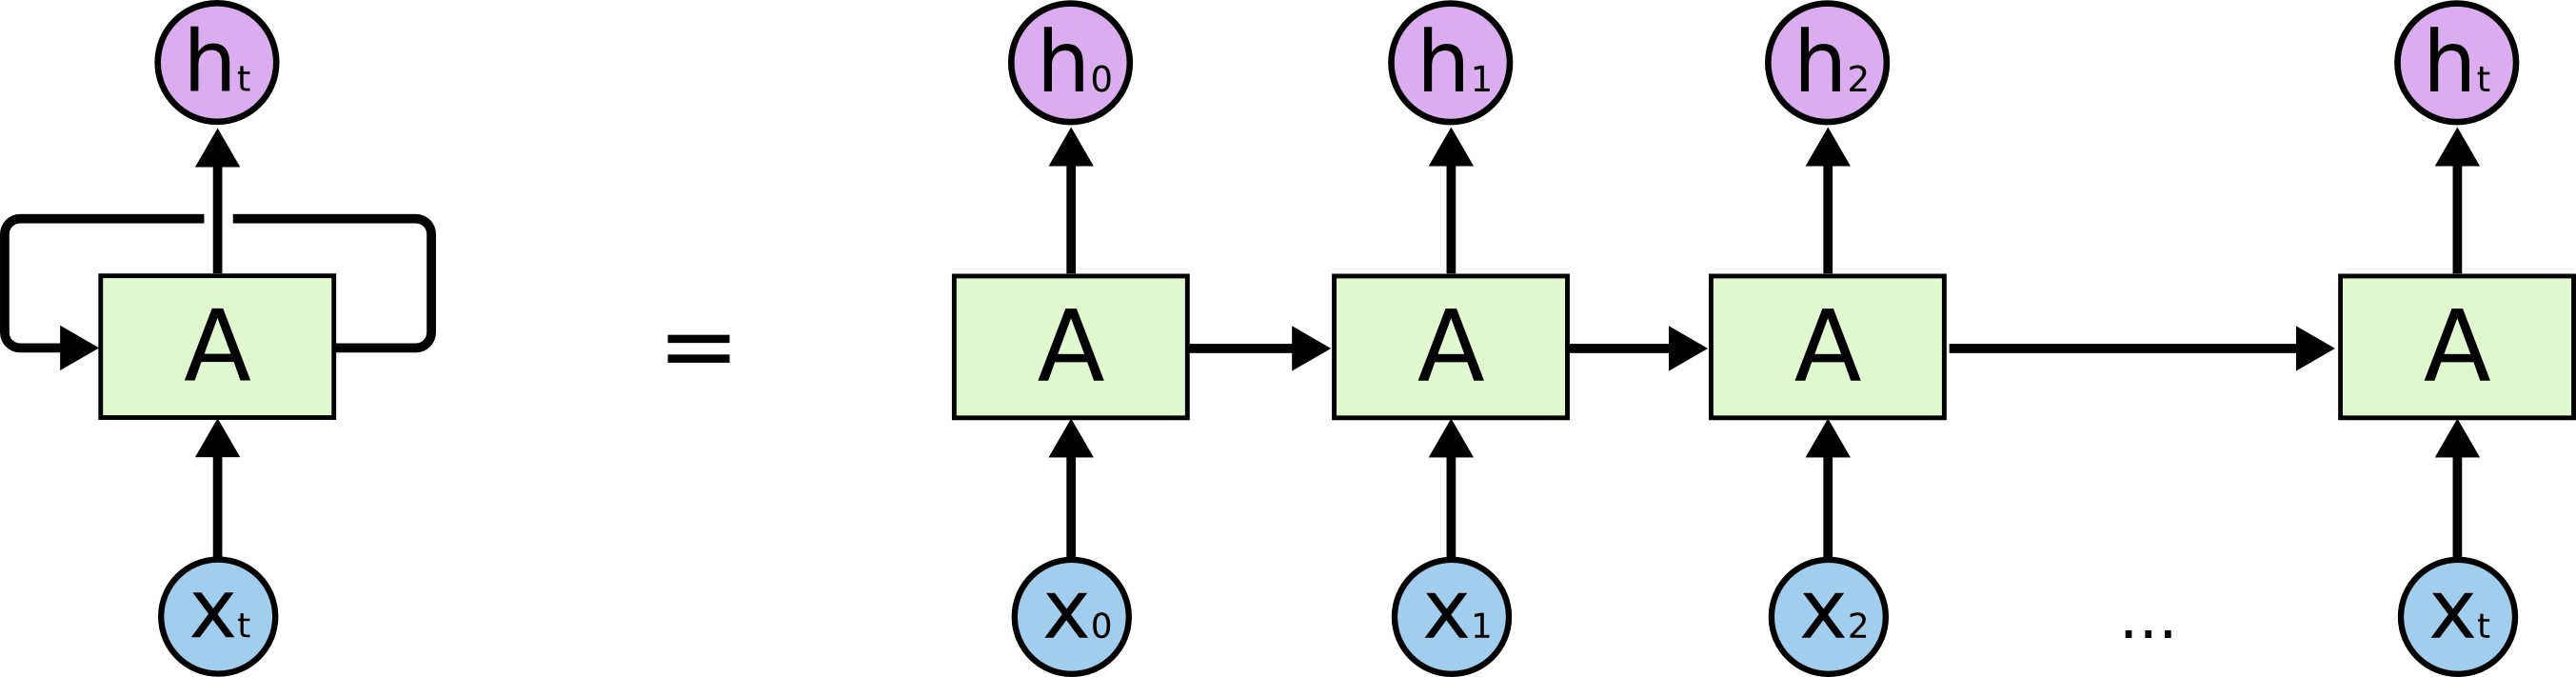
\includegraphics[scale=0.17,origin=c,]{images/RNN-unrolled.png}
		\label{fig:RNN-unrolled}
		
		Fonte: \url{http://colah.github.io/posts/2015-08-Understanding-LSTMs/}
	\end{figure}

	$\bullet$ Redes neurais recorrentes (RNN) \cite{elman1990finding}, são uma família de redes neurais que fazem o processamento de dados sequenciais, onde a dependência temporal é importante para o resultado \cite{Goodfellow2016}.
	
	$\bullet$ Devido à recorrência, um neurônio codifica uma sequência temporal.
	
	$\bullet$ O estudo em \citeonline{MikolovThesis2012} traz aplicações das RNNs aplicadas a modelagem da língua.
	
\end{frame}